
\subsection{Light Propagation}

The electromagnetic radiance is expressed through the flow of minute particles, or quanta, named \textit{photons} in the context of light. The energy of a single photon, \begin{equation}W = h \cdot v \: \textup{[J]}\end{equation}
is a product of the frequency $v \:\textup{[Hz]}$, and the Planck constant $h = 6.62607015 \cdot 10^{-34} 
\:\textup{J\:s}$, valid for every harmonically oscillating system.


%\subsubsection{Quantum Fluctuations of Light}

Photons arriving at each pixel can be approximated by a Poisson  distribution function and arrive at random times. The rate of the photon arrivals, i.e. the distribution of the photons, is however still dictated by the local light intensity, as seen in Figure  \ref{fig:photon}. 

%$$\mathbb{P}\left\{B_{m}=1 ; s_{m}\right\}=\mathbb{P}\left\{Y_{m} \geq q ; s_{m}\right\}=\sum_{k=q}^{\infty} \frac{s_{m}^{k} e^{-s_{m}}}{k !}$$

\begin{figure}[h]
  \centering
  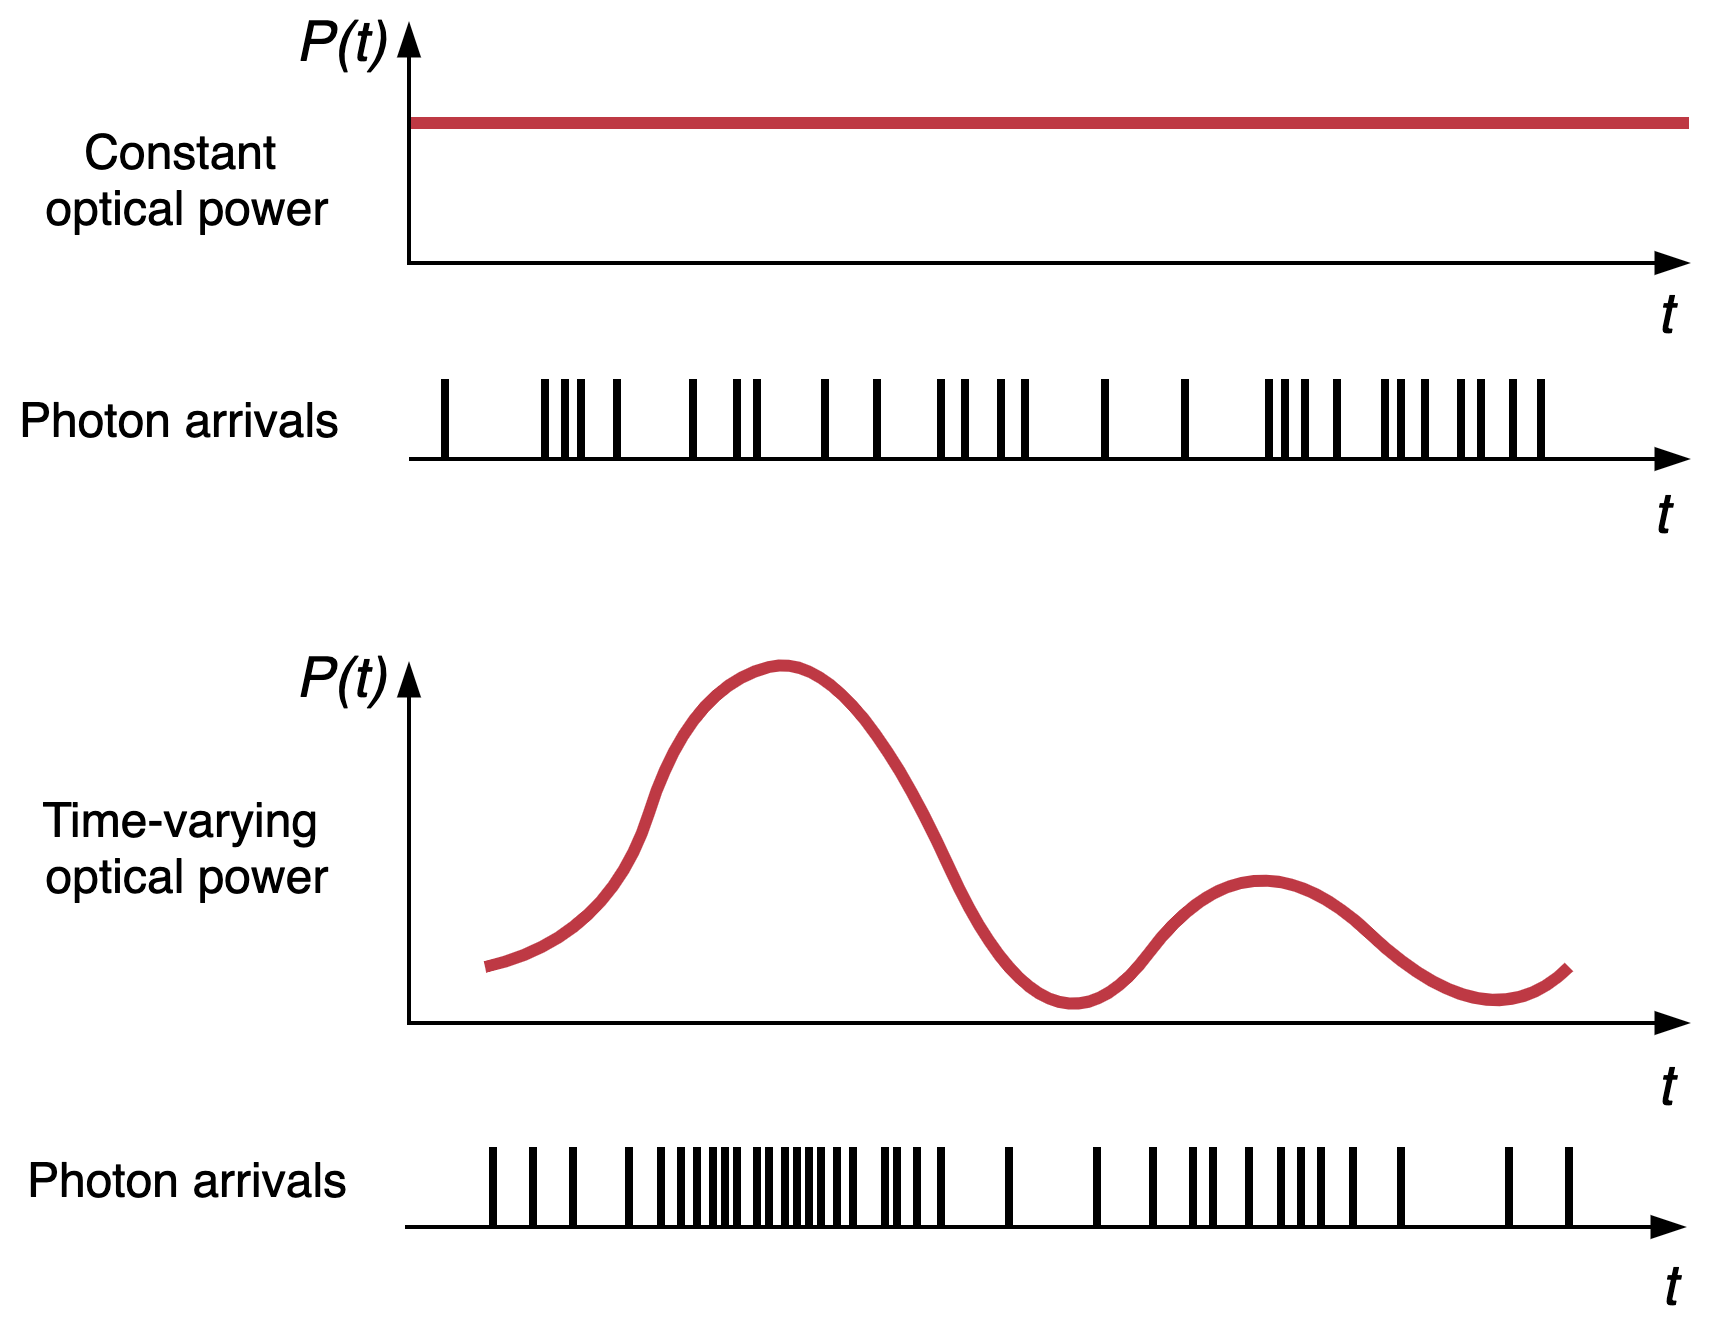
\includegraphics[width=\linewidth]{imgs/optics/photon.png}
  \caption{Random photon arrival time, modeled with two optical power sources. Even for a constant source, the arrival is probabilistic. Adapted from \cite{Saleh1991}.}
  \label{fig:photon}
  \Description{Two diagrams depicting behavior of registered photons in time depending on the variations in optical power.}
\end{figure}

\subsection{Photoelectric Effect in Sensors}

%The charge within each pixel on a sensor is collected through the estimation of the photons impinging on the respective pixel surface, inversely proportional to the capacitance ....
%A photon with energy hν breaks a silicon bond and frees both an electron (e-) and a hole (e+).
Imaging electronic devices consist of arrays of pixels, consisting of photodiodes accumulating charge through incoming light and integrated circuits which read out the charge and process it further.

For the accumulation of charge, the properties of the semiconductor materials are exploited. 
The unique electrical conductivity of semiconductors can be altered significantly through external sources of energy, e.g. thermally or by light illumination, and increases proportionally. 

The incident photons impinge on the surface of the image sensor and are absorbed through the corresponding structures in the semiconductor material, creating electron-hole pairs as the electron is excited from the valence to the conduction-band. The photoexcited carriers remain within the sample; this is called \textit{internal photoeffect}. \cite{Saleh1991} %645 & 576 %to the higher energy level.

Electrical and optical properties of the semiconductors can be altered further through \textit{doping}, an adding of local impurities for changed concentration of the carriers. In semiconductors, selective doping creates an electrostatic potential well. Subjected to the externally applied electric field, the freed photoelectrons drift through the material towards the potential well, where they are stored and integrated for the duration of exposure. This photoelectron charge is later transferred to the sense capacitance, thus producing measurable electric current through changes in the charge on the charge sense node (\textit{floating diffusion} FD) and converting the signal to voltage, which is read out by the a source follower transistor. \cite{9059308} %their charge is converted to voltage via transfer to a sense capacitance, change in the charge on this sense node causes change in voltage, thus converting the signal from charge domain to voltage domain

The outputs of the source-followers are amplified and fed to the signal processing circuits on a greater scale, allowing the separate pixels to be adressed column-wise. After the integration, the pixels are reset.

\begin{figure}[h]
  \centering
  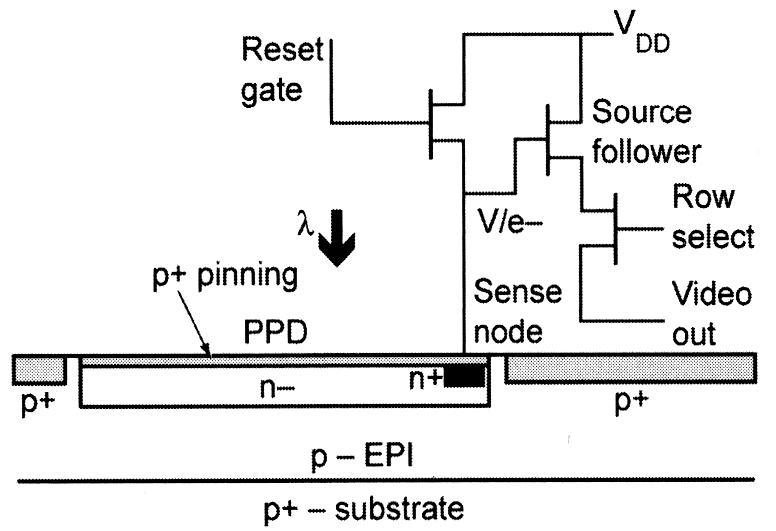
\includegraphics[width=0.9\linewidth]{imgs/sensors/3tppd.png}
  \caption{3T PPD structure, via \cite{Holst2011}. Typically, the dark current is heightened through the direct n+ contact; here, this is prevented through p+-pinning structure on the pixel surface.}
  \label{fig:3tppd}
  \Description{The classical pinned photodiode structure with three nodes.}
\end{figure}

Many implementations for the photodiodes exist. In the simplest pixel circuit, three transistors (3T: source-follower, reset, and row select transistors) are needed for the integration process. Modern CIS technologies make use of 4T pinned photodiode structure, in which an additional transfer gate is positioned between photodiode and the sense node. This ensures reduction of dark current and complete charge transfer; the ``pinning'' of the photodiode allows for reduced sense node capacitance. 
Furthermore, with this design structure, the pixels can be reset simultaneously, allowing for same integration periods globally.

\begin{figure}[h]
  \centering
  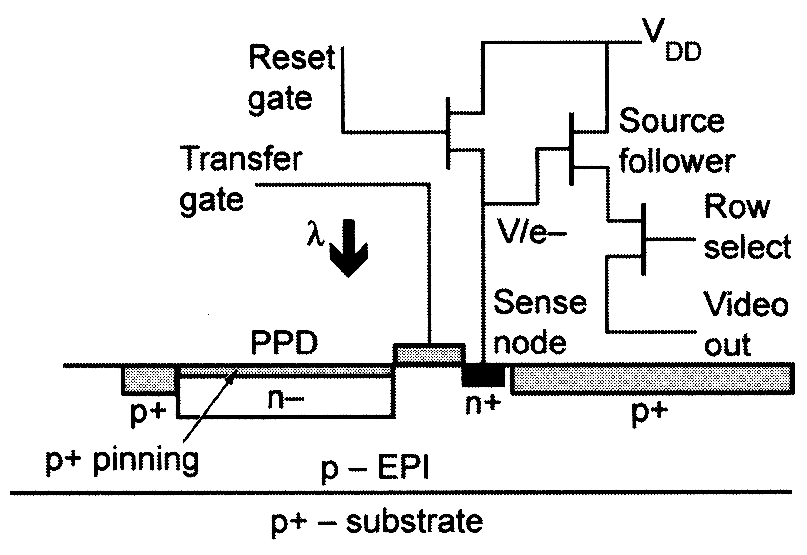
\includegraphics[width=0.9\linewidth]{imgs/sensors/4tppd.png}
  \caption{4T PPD structure, via \cite{Holst2011}. The transfer gate provides isolation of the regions.}
  \label{fig:4tccd}
  \Description{The pinned photodiode structure with four transistors. There are slight differences regarding the placement of the wells and the junctions, as the n+ is now spatially separated from the n-.}
\end{figure}

Only a fraction of the incident photon flux is absorbed and brought to a higher energy level. The ratio of the photoelectrons to the incident photons is given by \textit{quantum efficiency} (QE), which often ranges from 50\% to 80\% \cite{9059308}.
The relationship between the changes in output voltage caused by the photoelectric effect to the number of photoelectrons is given by conversion gain (CG); in modern CIS devices, this typically amounts to 100$\mu$V/$e^{-}$~\cite{7006672}. 


\subsection{Noise Modeling in Digital Sensors}


The noise, that is, unwanted deviations in the signal, can be comprised of the multiple sources which are subsequently added throughout the digital image acquisition chain. Deviations in the brightness are introduced right in the detection phase due to the discrete nature of electrons; such noise source is dubbed photon shot noise. Further fluctuations are caused during the readout of the electron charge and its subsequent amplification; for digital systems, the mapping of the voltage to discretized bit values results in the additional quantization noise. \cite{Holst2011}

\begin{figure}[h]
  \centering
  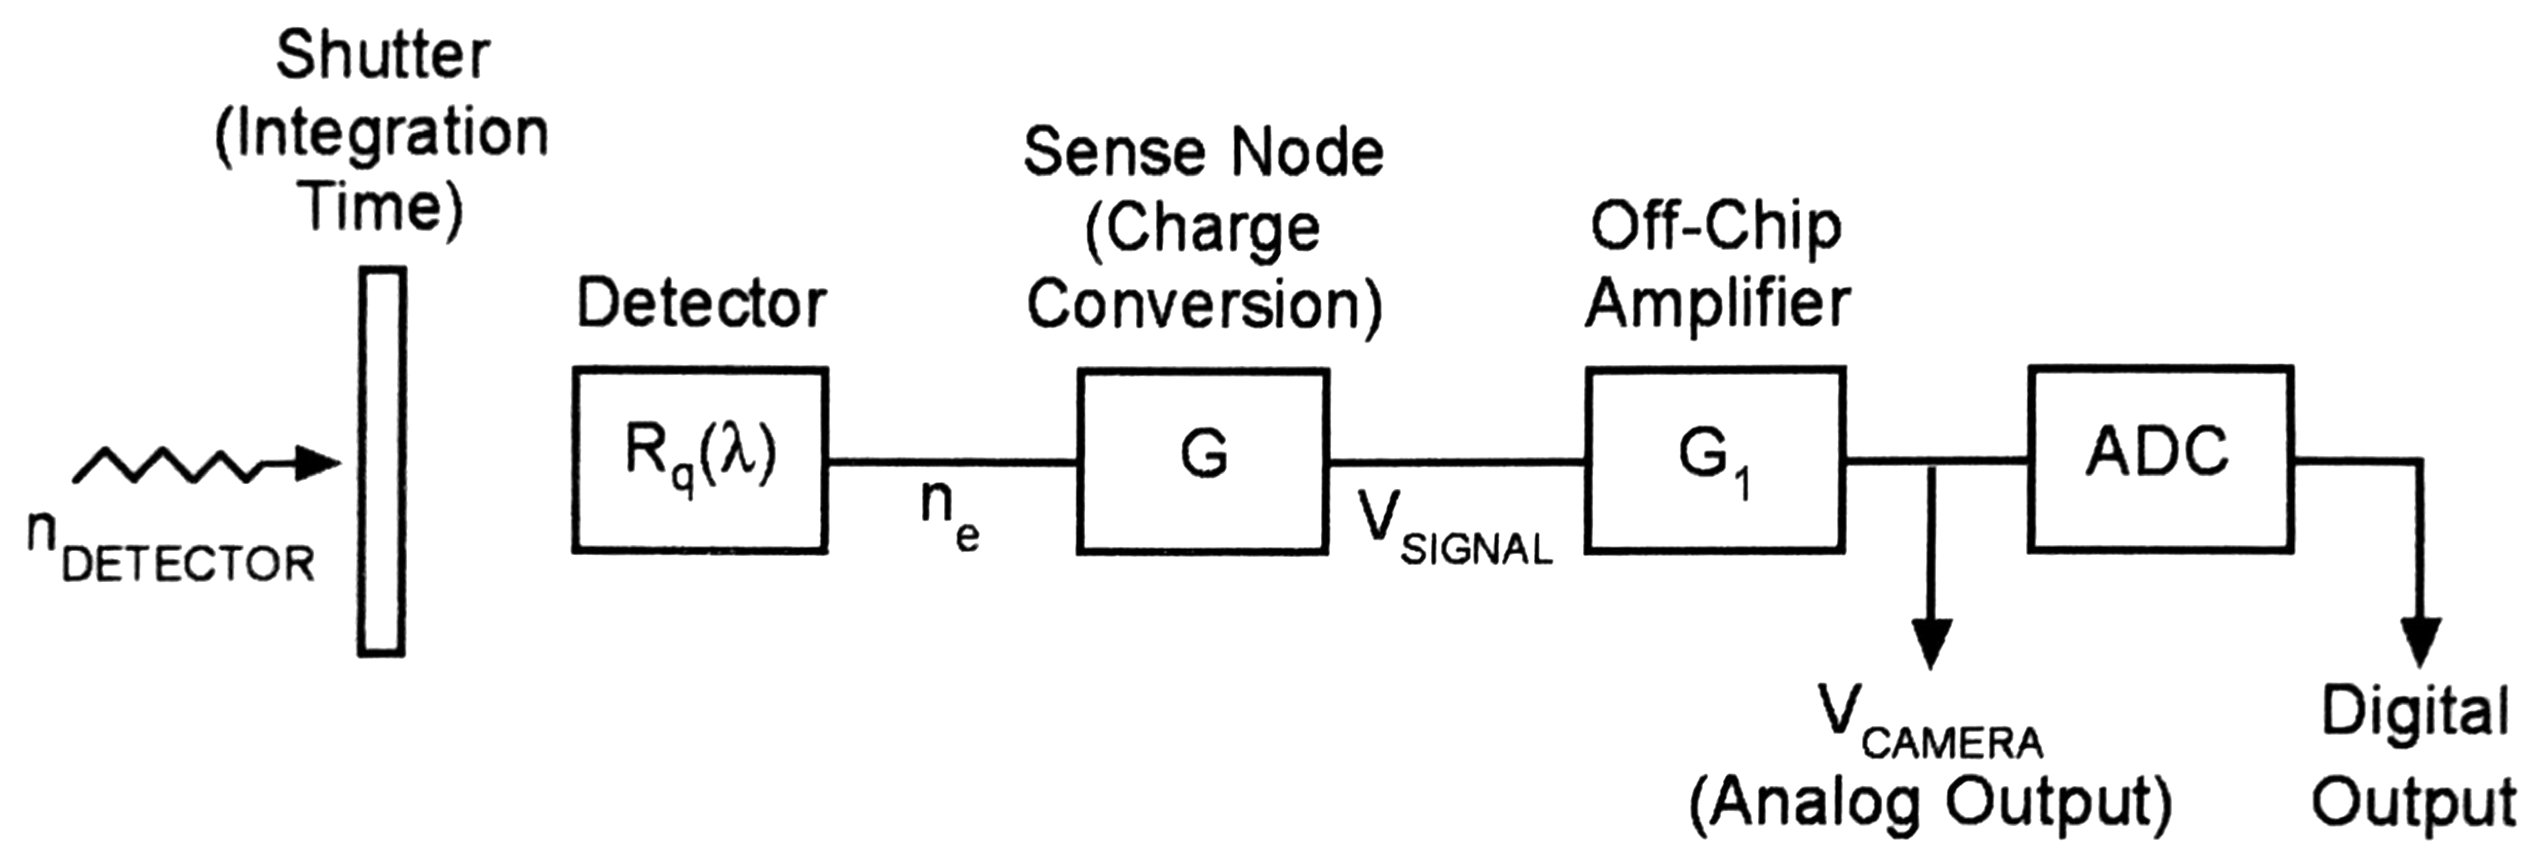
\includegraphics[width=\linewidth]{imgs/sensors/sens-signal-transfer.png}
  \caption{Signal transfer diagram in an imager, via \cite{Holst2011}. Both analog and digital outputs are considered.}
  \label{fig:sigtrans}
  \Description{Signal transfer diagram in a digital sensor. There are multiple subsystems leading to the accurate normalized representation of the signal: at first, the incident photons are detected and evaluated in their charges; this is later amplified and digitized.}
\end{figure}

\begin{figure}[h]
  \centering
  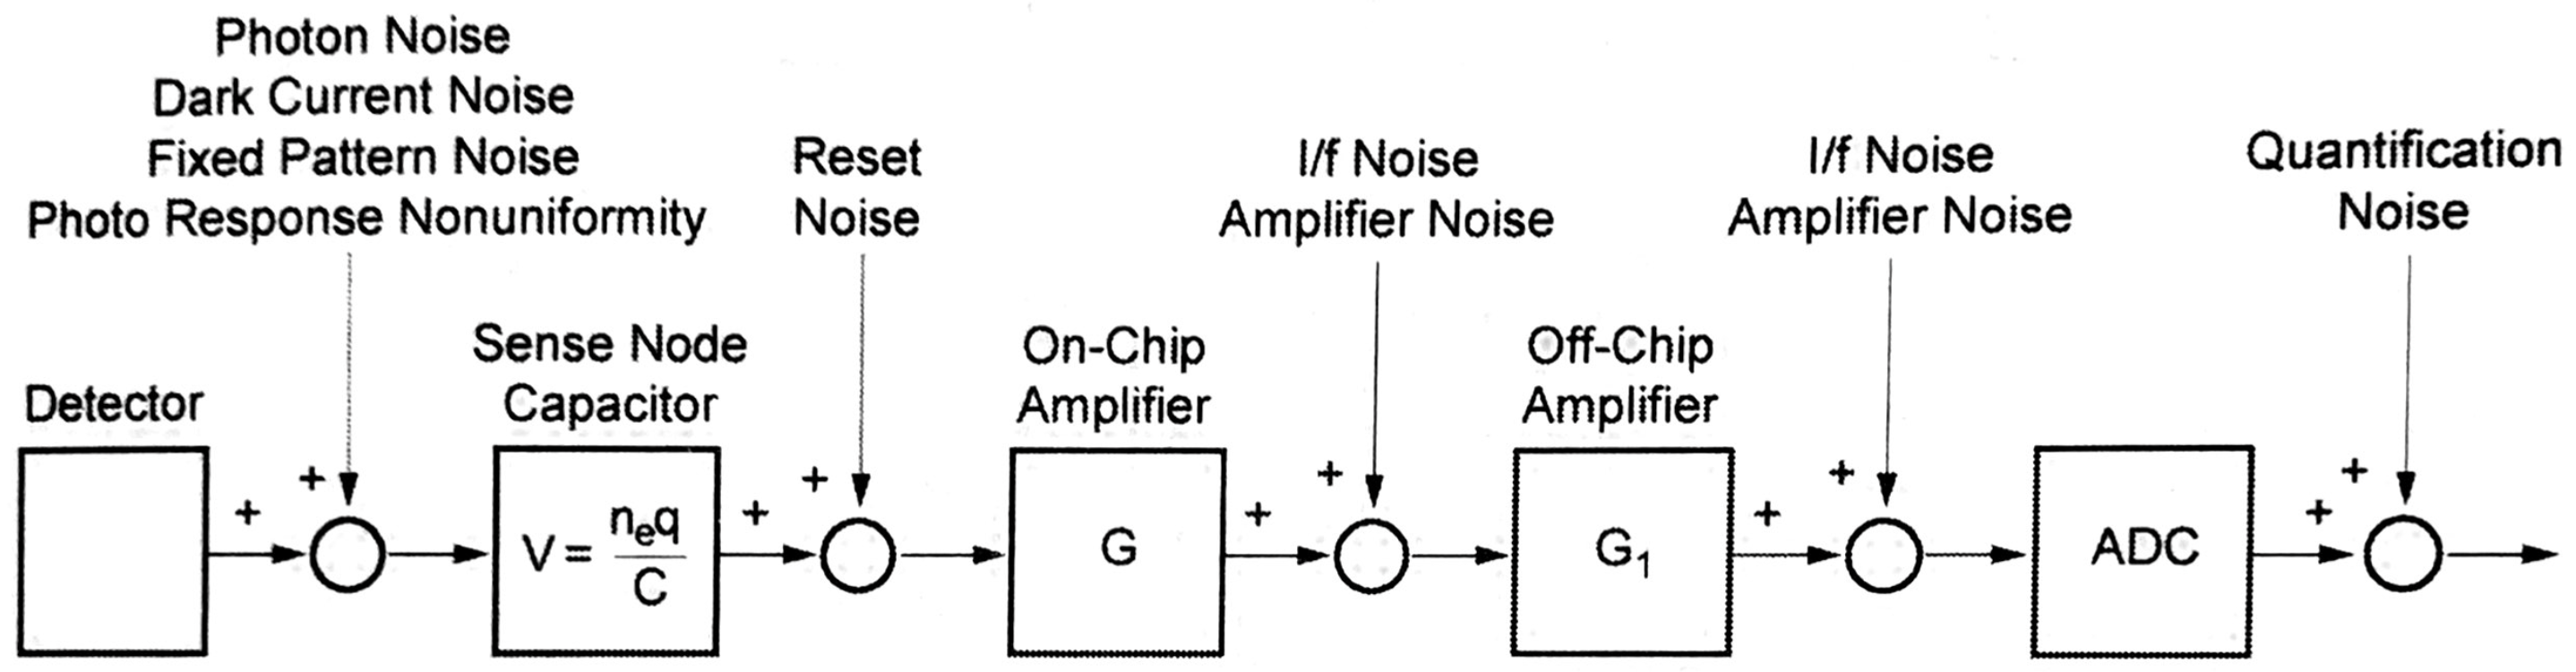
\includegraphics[width=\linewidth]{imgs/sensors/sens-noise-transfer.png}
  \caption{Noise transfer in a digital sensor, via \cite{Holst2011}. Each subsystem introduces additional noise sources which affect the subsequent signal.}
  \label{fig:noisetrans}
  \Description{For every subsystem listed in the signal transfer diagram, there is a corresponding noise source which alters the input: the photon-induced noises, reset noises, noises caused through amplifiers (off-chip and on-chip), and finally, the quanification noise.}
\end{figure}

Figures \ref{fig:sigtrans} and \ref{fig:noisetrans} show the signal transfer and the noise occuring during each step of the process, respectively. Each noise source has a different characteristics and can be attributed to either nonuniformities and physical flows of the sensor, or the natural nonstationary processes. The level of detail in the noise transfer diagram is somewhat dependent on the application, and some of the sources caused by the circuitry can be minimized through the design of the architecture, as will be shown in the further chapters. 

\subsection{General Requirements in Gigapixel Applications}

Several general requirements must be met in gigapixel imaging devices. Since the higher information efficiency is desired in both scientific and consumer-grade applications (see Section \ref{chapter:motivation}), a high-resolution camera must not differ drastically from current implementations in its imaging capability.

For components which are primarily influenced by optoelectrics, \cite{GigaOptik} name following requirements:

\begin{itemize}
    \item a \textit{field of view} (FOV) of at least ca. 40$^\circ$, which is equivalent to the angle of view for humans at infinity focus ($\mathrm{FOV} = 2 \times \arctan\left(\frac{\text{sensor size}}{2{f}'}\right)$, ${f}' = 50m$m),
    \item an f-stop of ca. f/4-f/11 for operation under most common lighting conditions,
    \item and a lens design with low complexity to facilitate both portability and low manufacturing costs.
\end{itemize}

\subsection{Diffraction-Limited Systems}% (→ comparison with classical optics)

\label{chapter:diff}

In a typical imaging system, before arriving at the sensor, the incident light is collected and focused through an optical system first. Lenses, most common optical components, have a resolving power of their own, which has to match the resolution of the sensor and is fundamentally limited by the nature of light. 

Upon encountering an opening (\textit{aperture}), the incident light diffracts into a series of concentric waves propagated concentrically around the corners. Assuming a perfectly circular aperture, wavefronts belonging to one point in object space will produce a diffraction pattern with a bright spot in the middle, surrounded by concentrical rings of reduced intensities. The diameter of such pattern, \textit{Airy disk}, is given through:

\begin{displaymath}
    D_{Airy} \approx 2.44 \frac{\lambda {f}'}{D} = 2.44 \lambda  k
\end{displaymath}

with $\lambda$ being the wavelength of the incoming light, ${f}'$ the focal length, and $D$ the diameter of the entrance pupil, respectively; in lenses, which can be treated as a circular aperture of respective diameter, the \textit{focal ratio} serves as the \textit{nominal aperture} $k$, or \textit{f-stop}. 

\begin{figure}[h]
  \centering
  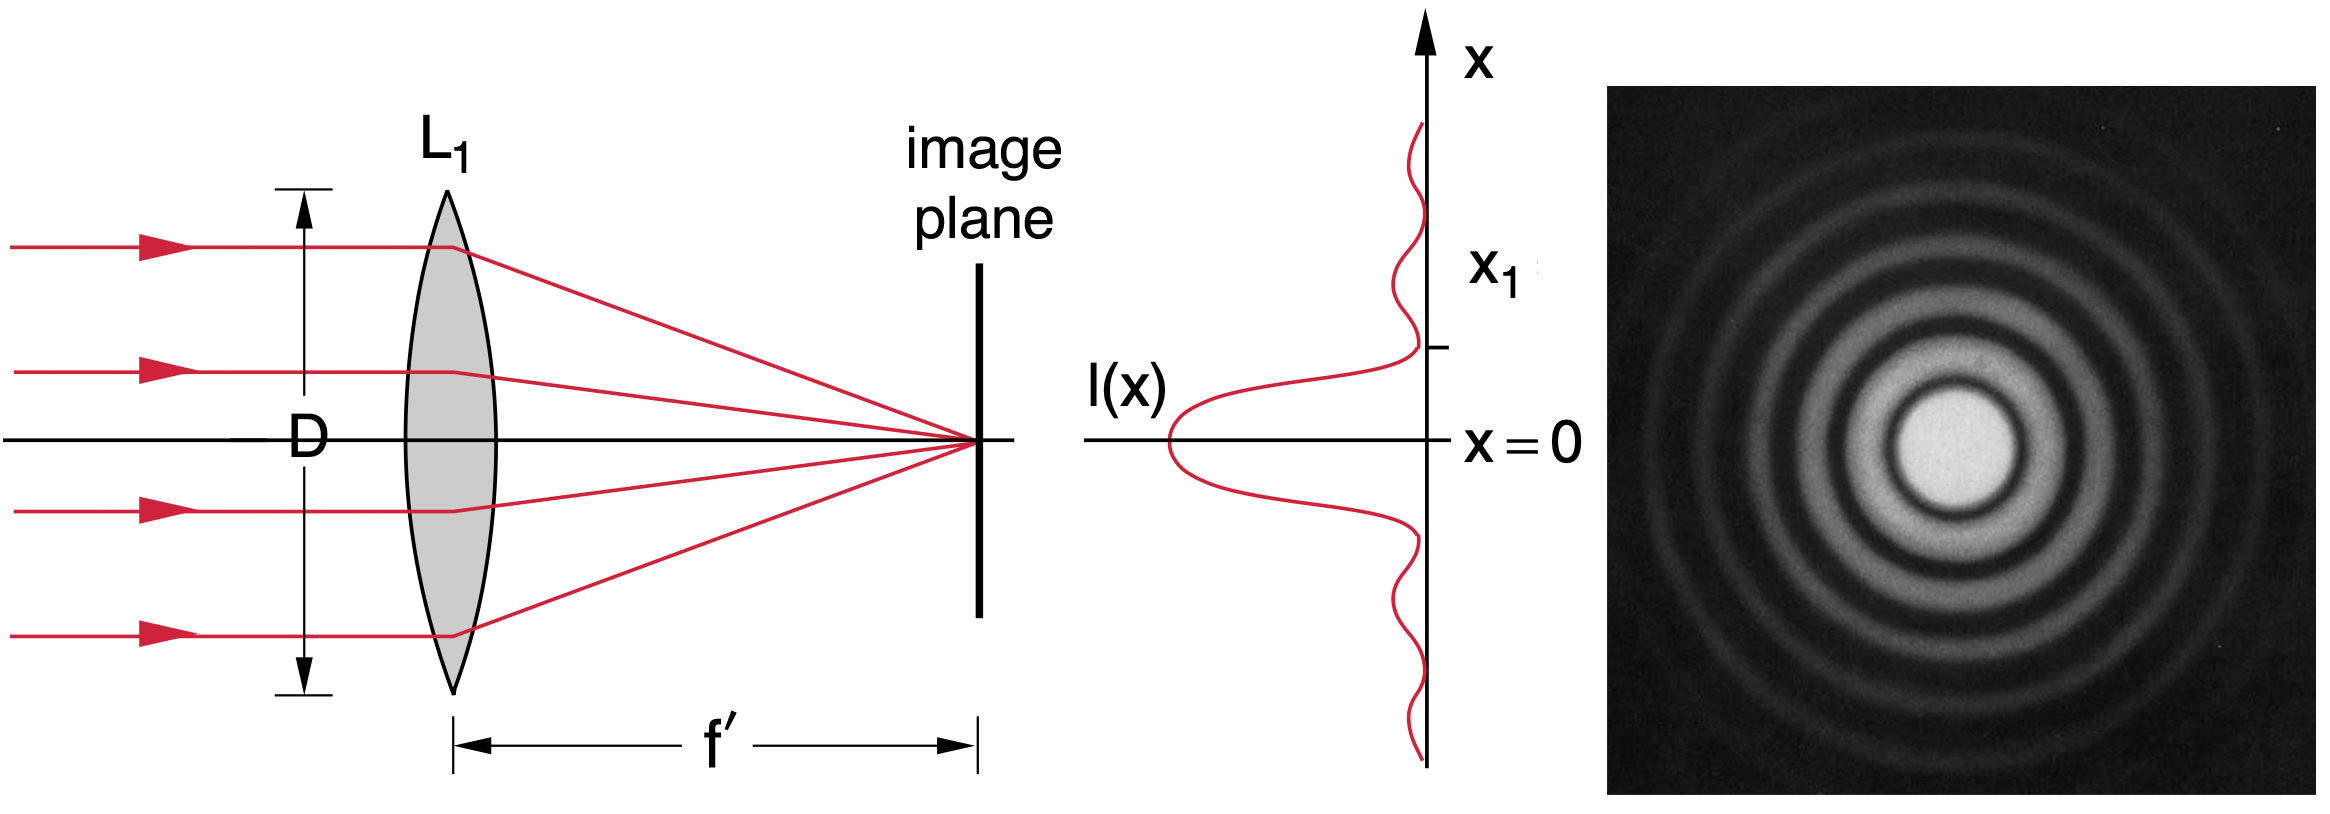
\includegraphics[width=\linewidth]{imgs/optics/airy.png}
  \caption{Airy disk pattern caused through lens diffraction of a point source, via \cite{Cagnet1962}, and and the corresponding distribution of intensities, \cite{Demtroeder2018}.}
  \label{fig:airy}
  \Description{The bundle of light passing through a lens, acting as an aperture. Through diffraction, the points in the object plane are depicted as a concentric wave-like pattern of diminishing intensities.}
\end{figure}

For two distant neighboring points, the half-angle ${\delta}'_{min}$ subtended by the numerical aperture (represented by the lens) is too small. Thus, the two objects will not be perceived as separate entities; as their intensity functions coincide at their respective minimums, the disks will start to overlap. 

\begin{figure}[h]
  \centering
  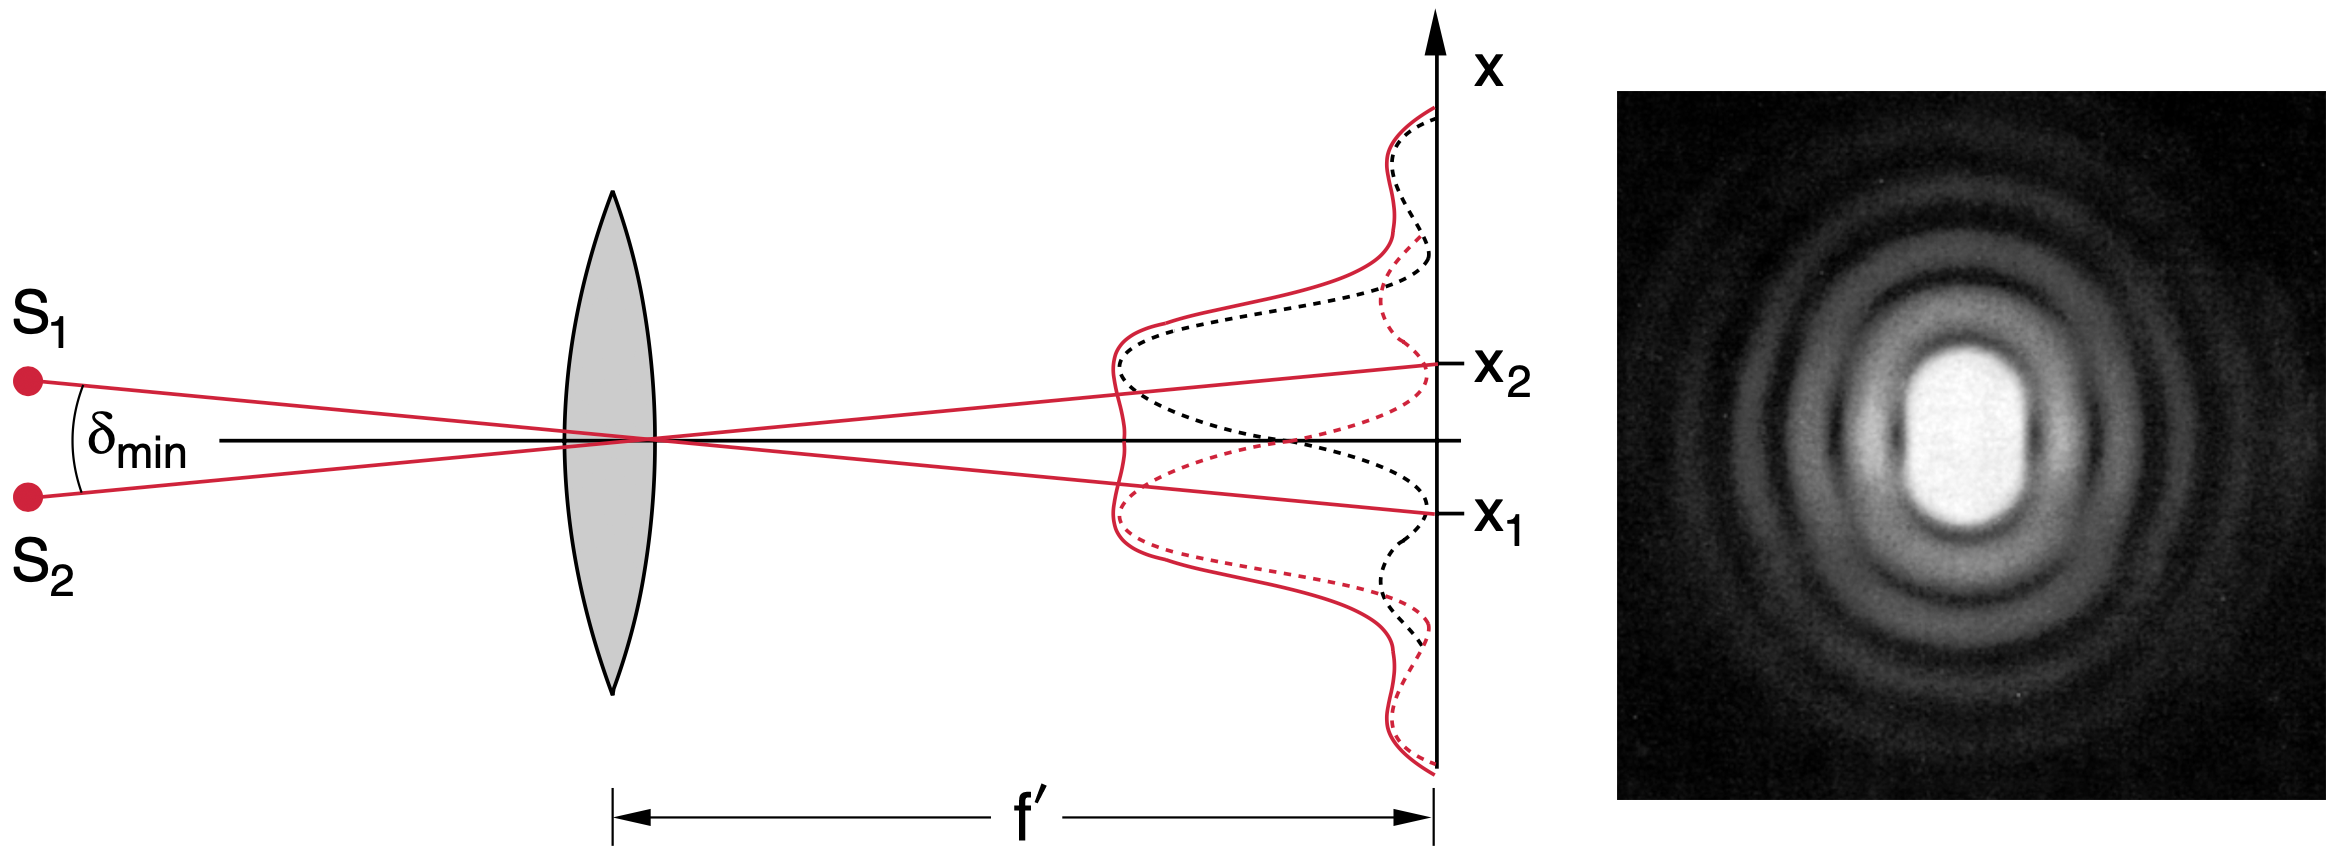
\includegraphics[width=\linewidth]{imgs/optics/airy-limit.png}
  \caption{The imaging subsystem is not capable of resolving two adjacent object points, leading to the interferences in the signal. Via \cite{Cagnet1962} and \cite{Demtroeder2018}.}
  \label{fig:airylimit}
  \Description{Two point sources are depicted in an imaging system and raytraced in a manner similar to the previous figure. The limits placed by diffraction cause the concentric patterns to overlap, rendering the two point sources spatially indistinguishable from each other.}
\end{figure}
%also, numerical aperture = n sin delta, with n = 1 bc air
The angular resolution of an optical system in an object plane is concomitant with a spatial resolution in an image representation, due to to the small-angle aproximations \cite{Pedrotti2007}. Defined via \textit{Rayleigh criterion}, the least resolvable distance between two points should correlate with the distance between the two peaks of the intensity distribution function (as seen in Figure \ref{fig:airylimit}):

\begin{displaymath}
  {\delta}'_{min} =  1.22 \lambda \frac{{f}'}{D} = 1.22 \lambda k \simeq {\rho}'_{\infty } 
\end{displaymath}

The latter is defined as the resolution limit ${\rho}'_{\infty}$ and can be approximated for the near field application, where the distance ${a}'$ between the aperture and the sensor plane is larger than the focal length ${f}'$:

\begin{displaymath}
{\rho}'_{near}  =  1.22 \lambda \frac{{f}'}{D} \frac{{a}'}{{f}'}= 1.22 \lambda k (1 - {\beta}' )
\end{displaymath}

The resolution limit presented earlier sets a limit for the peak lens performance, which varies with the fundamental physical quantities, like wavelength range and focal ratio.  
Further limitations are imposed through the geometric aberrations, caused by the physical imperfections in the optics itself.

The number of distinct resolvable points for a lens is defined by the \textit{space-bandwidth product} (SBP) \cite{Cossairt:11} and ties the lens performance to the sensor size.

\cite{GigaOptik} state two common approaches for enhancing the SBP. Those consist of either scaling the system up, or introducing further optical surfaces to the imaging system for better lens performance. The scaling can occur in either one of the subsystems, meaning an integration of a sensor with larger dimensions or scaling the lens.%, which are said to have SBP quadratic... aus scaling laws 
The second measure should lessen influence of geometric aberrations, leading to a diffraction-limited performance; however, the increased complexity of the optical system implies higher manufacturing costs and errors due to misalignment. Detailed description of scaling laws for the lenses is provided in \cite{Cossairt:11}, who account for both diffraction-induced limits and geometric aberrations.

As the CIS pixel sizes are routinely surpassing the 1.5$\mu$m extent, the optical system in a gigapixel application is doomed to have a lower resolving power than the sensor itself even if the lens performance is solely diffraction-limited; hence, the resolution in image space will be limited through optics. Resulting image representations contain spatial redundancies due to the light field being oversampled. 

While many proof-of-concept solutions exist that aim to enhance the resolution on a solely optical level (i.e., multiscale design and monocentric lenses), computational post-processing in gigapixel devices might turn out to be compulsory.
